%!TEX root = thesis.tex
\chapter{Introduction}
\label{cha:introduction}

Ever since the dawn of time, the humankind have looked at the stars and wondered if we are alone in
this Universe. To answer this question, one must look toward the field of extrasolar planets
(exoplanets). This is a rapidly growing field in astronomy and science in general. Ever since the
first confirmed discovery of an exoplanet around a millisecond pulsar in 1992 by
\citet{Wolszczan1992} and three years later, the more interesting exoplanet 51 Peg b discovered
around a solar-type star by \citet{Mayor1995}, more than 3600 exoplanets have been discovered at the
time of writing, July 2017\footnote{\url{http://exoplanet.eu/}}.

With the discoveries of exoplanets, the main focus of observational exoplanetology is now mainly on
finding the twin of Earth; that is a planet that can harbour life as we know it. The Earth twin will
be of similar size (both in mass and radius), and be located in a distance from its host star were
liquid water may exists on the surface. When speaking of detecting life, it is important to note
that it is the biosignatures that life will cause on the exoplanet's atmosphere that the astronomers
are and will be looking for. Before even start the search for these biosignatures on another
exoplanet, the exoplanet must be carefully characterised so we do not end up looking blindly for the
biosignatures. Additionally, it may not be necessary to find an Earth replica in order to find
conditions for life (see e.g. \citet{Alibert2014} for a discussion on habitable planets unlike the
Earth). Lastly, are the compositions and origins interesting in this era of exoplanetary science.
However, in order to accurately and precisely characterise an exoplanet, it is is crucial to
characterise its host star. This is commonly known as ``know the star, to know the exoplanet''. It
is possible to obtain planetary global parameters such as its radius and mass if the stellar
parameters are accurately known. With high precision it is even possible to distinguish between
different planetary bulk compositions such as water-worlds, rocky planets, gaseous planets, iron
planets, or exotic combinations of the above \citep[see e.g.][]{Dorn2015,Thiabaud2014}.

In this chapter there will be a general introduction to exoplanets, detection methods, and
characterisation (\sref{sec:exoplanets}). Then a throughout introduction on the exoplanet host stars
(\sref{sec:planet_host_stars}), which is the main focus of this thesis. In the end of this chapter,
the importance of stellar studies will be discussed along with its wide-spread applications
(\sref{sec:stars_application}) before a general overview of this thesis (\sref{sec:this_thesis}).



\section{Exoplanets}
\label{sec:exoplanets}

The holy grail in the field of exoplanets is to find the first exoplanet with biosignatures. This is
by no means an easy task. To give an idea of the difficulty of detecting biosignatures on an
exoplanet, it is important to understand all the difficulties when simply detect and confirm an
exoplanet. This will shortly be described in the sections below where several detection techniques
will be introduced.

\subsection{Detecting exoplanets}
\label{sec:detecting_exoplanets}

There are six main techniques for detecting exoplanets, some with advantages over others. These
advantages depends strongly on the advancement of the instruments used for the different techniques,
but also on the physical properties of the exoplanetary system. A lot of information about the
exoplanets can be extracted when more than one of techniques are used and combined. The success of
the different methods can be seen in \fref{fig:detectionTypes}, Where all the detected planets (with
measured masses) are shown divided into which group was used for detecting the exoplanets. The most
exoplanets are discovered with the transit method and the radial velocity method, both which will be
explained in more detail below. Additionally, the figure also include Mercury, Earth, and Jupiter
(size of the symbols are not to scales).

\begin{figure}[htpb!]
    \centering
    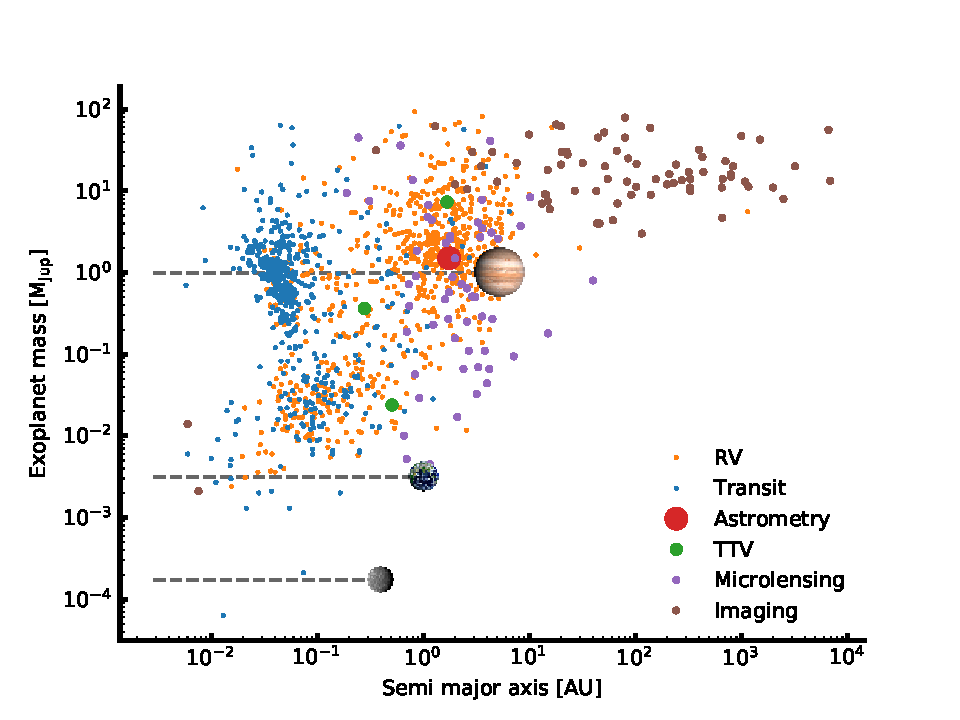
\includegraphics[width=1.0\linewidth]{figures/exoplanetDetectionType.pdf}
    \caption{Confirmed exoplanets with the derived masses (relative to Jupiter) and the semi-major
             axis. The position of Mercury, Earth, and Jupiter are also shown, however the symbols
             are not to scale. The size of the symbols for the different detection methods are
             different in order to clearly see the methods which did not yet detect many exoplanets
             such as \emph{Imaging} or \emph{Astrometry}.}
    \label{fig:detectionTypes}
\end{figure}

It is important to note, that different phenomena might mimic planetary signals, such as stellar
activity, or the contaminating light from a fainter stellar companion \citep[see
e.g.][]{Queloz2001,Oshagh2013,Oshagh2014}. However, they will not be described in this thesis.  The
description of the different detection techniques are inspired by \citet{Seager2010}.


\subsubsection{Transit method}
\label{sec:transitMethod}

The most successful method, if based on numbers of exoplanets detected, is the transit method. The
integrated light of a star is continuously monitored in order to detect a transit. This kind of data
is called a photometric time-series, and have wide applications in stellar astrophysics. It is not
enough to monitor a star to detect a transiting exoplanet. It has to be aligned with the line of
sight from the observer, thus the probability of detecting exoplanets depends on the geometry of the
system.

Transit photometry is a well-known method in astronomy, however only used recently for detecting
exoplanets. Before this, it has been used extensively for finding and characterising eclipsing
binary stars. The difference here is, that the exoplanet is extremely small and does not radiate (or
at least emit very little radiation). An example of an exoplanet transiting a star can be seen in
\fref{fig:transitMethod} for K2-29 b. The data is from a summer school\footnote{Data can be found
here: \url{https://github.com/iastro-pt/AzoresTE1}}, which was prepared from \citet{Santerne2016}.
The data below in \sref{sec:rvmethod} is from the same source.

\begin{figure}[htpb!]
    \centering
    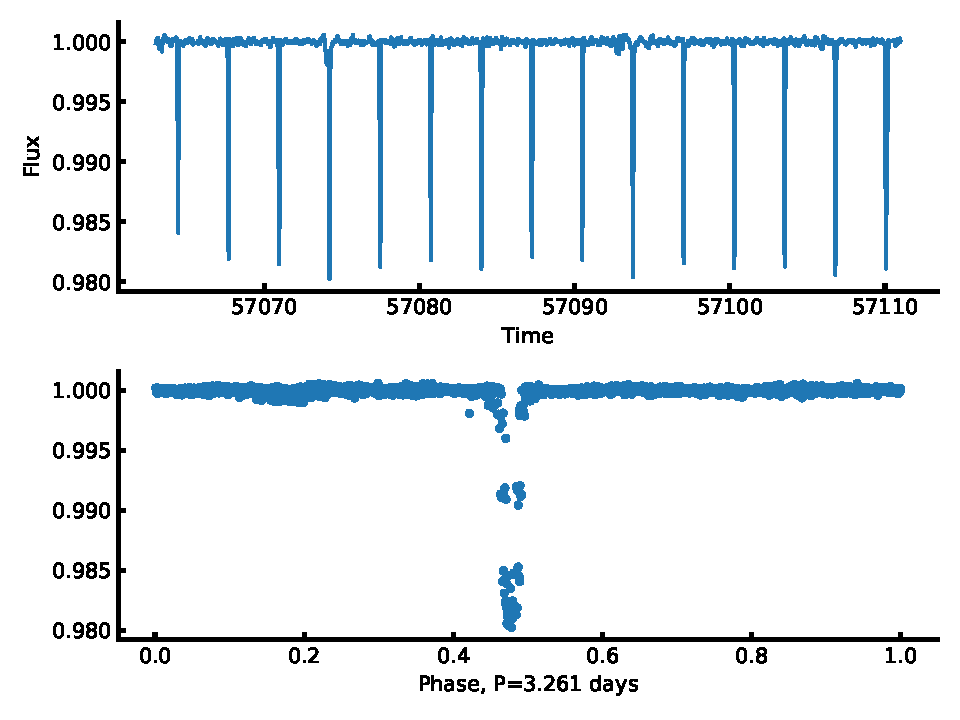
\includegraphics[width=1.0\linewidth]{figures/transitMethod.pdf}
    \caption{\emph{Upper plot}: The lightcurve of a star with an exoplanet transiting.
             \emph{Lower plot}: The phase curve of the above lightcurve using the period of
             \SI{3.259}{days}.}
    \label{fig:transitMethod}
\end{figure}

When an exoplanet transits its host star, the total brightness from the system will decrease, as the
exoplanet blocks some of the light from the star. This dimming in brightness will be seen
periodically as the exoplanet orbits its host star. The decrease in brightness as the planet transit
the star is directly related to the ratio between the stellar radius $R_\ast$ and the planetary
radius $R_p$:
\begin{align}
  k = \sqrt{\frac{R_p}{R_\ast}},  \label{eq:transit}
\end{align}
where $k$ is the depth of the transit compared to the normalised stellar brightness.

This method allows to determine the radius of the planet as far as the radius of the star is known.
Furthermore, detailed analysis of the phase curve of an exoplanet can additionally reveal the
surface temperature of the exoplanet. The transit described above is also known as the primary
transit. During secondary transit, that is when the exoplanet goes behind the star as seen from
Earth, the flux of the exoplanet will be observed. The flux of the exoplanet is a measure of the
surface temperature. It is difficult to observe secondary transits. This is mainly due to the low
flux from the exoplanet.



\subsubsection{Radial velocity method}
\label{sec:rvmethod}

The radial velocity method is the study of the motion of the host star using the Doppler effect
caused by an orbiting exoplanet\footnote{As the transit method, this method has been known for
decades in the study of e.g. binary stars.}. This together with the transit method described above
are by far the most successful methods to detect and characterise exoplanets  with the current
instruments. The periodic signal created by the exoplanet on the host star depends on the mass ratio
between the star $M_\ast$ and the planet $M_p$:
\begin{align}
  K = \frac{\SI{28.4329}{m/s}}{\sqrt{1-e^2}} \frac{M_p\sin i}{\Mjup} \left( \frac{M_\ast+M_p}{M_\odot} \right)^{-2/3} \left(\frac{P}{\SI{1}{year}}\right)  \label{eq:rv}
\end{align}
where $K$ is the semi-amplitude of the sinusoidal, $e$ is the eccentricity, $i$ is the inclination
of the orbital plane compared to the line of sight from Earth, $P$ is the orbital period, and
$\Mjup$ is the mass of Jupiter. Since $M_\ast \gg M_p$, the term $M_\ast+M_p\simeq M_\ast$ in order
to simplify the equation. Often a circular orbit is assumed, hence $e=0$. The sinusoidal motion of
the star can be seen in \fref{fig:rvmethod} where both the time series and the phase curve is
presented for the exoplanet, K2-29 b.

\begin{figure}[htpb!]
    \centering
    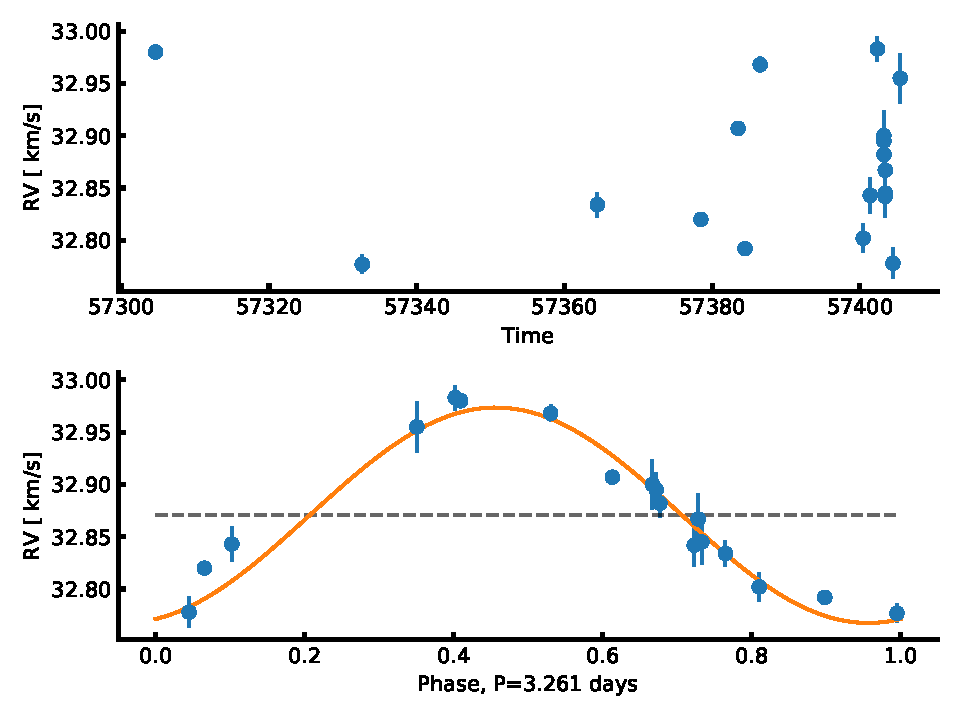
\includegraphics[width=1.0\linewidth]{figures/RVmethod.pdf}
    \caption{\emph{Upper panel}: RV time series of K2-29 b from the SOPHIE spectrograph.
             \emph{Lower panel}: Phase curve of the time series above, using the period of
             \SI{3.259}{days}. The fit is a simplistic sinusoidal for visual guidance.}
    \label{fig:rvmethod}
\end{figure}

In order to apply the radial velocity method for detecting exoplanets, it is necessary to collect
spectra (high resolution but often not high signal-to-noise ratio) in order to cover most part of
the phase of the orbit. These spectra are often combined after the detection of the exoplanet, in
order to increase the signal-to-noise (S/N). This combined spectrum can then be used for
characterising the host star, which will be introduced below.


\subsubsection{Other techniques}

The following four techniques have all detected exoplanets, however, they are currently not widely
used and neither have the same level of success as the two methods described above. This is
something that will change in the future with new and up-coming instruments.

\paragraph{Direct imaging}

Direct imaging is probably the easiest method to understand, however it is quite difficult to
actually use this technique. In its core, by carefully blocking the light of a star, it is possible
to directly image the exoplanets around it. However, it is extremely difficult to block the light of
the host star and find the reflected light of the exoplanet(s) in orbit. One has to deal with
residual light from the host star, which are orders of magnitudes brighter than the exoplanets. With
SPHERE at VLT it is expected than more exoplanets will be found with this technique
\citep{Beuzit2008}.


\paragraph{Astrometry}

Using astrometry to detect exoplanets is very similar to the RV method described above in
\sref{sec:rvmethod}. Unlike the RV method, this technique (astrometry) actually looks for the minute
changes in the coordinates of the star, i.e. the direct movement of the star on the sky as seen from
Earth. The Gaia mission \citep{GAIA} will provide many exoplanets detected with astrometry.

This technique is sensitive to massive exoplanets as they cause a larger motion compared to lighter
companions.


\paragraph{Transit timing variation}

This technique of detecting exoplanets is a highly indirect method of detecting exoplanets. Here a
transiting exoplanet has to be detected first as explained in \sref{sec:transitMethod}. Then
variations in the occurrence of mid-transit can be detected if a second non-transiting exoplanet
interact with the primary transiting exoplanet (known as planet-planet interaction). This
interaction will periodically cause the mid-transit to happen ahead/behind of the time if only one
exoplanet would be present.

A careful analysis of the transit timing variations (TTV) can give the mass of the secondary
non-transiting exoplanet. However, its radius will be unknown. Most of these exoplanets pairs which
shows TTV are in an orbital resonance. This technique as well, is more sensitive to massive
exoplanets as they will induce a higher signal. However, it is also sensitive to exoplanets with
comparable semi-major-amplitudes.


\paragraph{Microlensing}

This technique is very exotic and not widely used, however since a few exoplanets have been
discovered by this technique it deserves to be mentioned. The core theory in this technique is the
well-known General Relativity by \citet{Einstein1916}. With this method an observer looks at a
distant star as a star between the observer and the distant star passes in between the line of
sight. The intermediate star will act as a lens and increase the magnitude of the distant star. This
increase of magnitude will reach its maximum as the two stars are most aligned as seen from Earth.

To use this method for detecting exoplanet, there will have to be an exoplanet orbiting intermediate
star. The exoplanet act as a microlens, momentarily make a secondary increase in magnitude. The
amount of increase in magnitude is related to the mass of the exoplanet. The higher the mass, the
higher the effect.

While this exotic technique is interesting and has detected exoplanets, it is not very useful as it
only occurs once. The stars observed with this technique are often faint, thus making follow-up RV
detection very difficult if not impossible with the current instruments.


\subsection{Towards the Earth twin}

The above mentioned techniques will be used to find the Earth twin. Especially will the two first
techniques (transit and RV method) be the ones finding the smallest exoplanets as a wide range of
instruments are being developed dedicated for this. Since the detection of the first exoplanet
around a solar-type star by \citet{Mayor1995}, the community has been able to detect lower mass
exoplanets as seen in \fref{fig:exoplanetMass} and the regime of Earth-mass exoplanets have been
reached very recently.

\begin{figure}[htpb!]
    \centering
    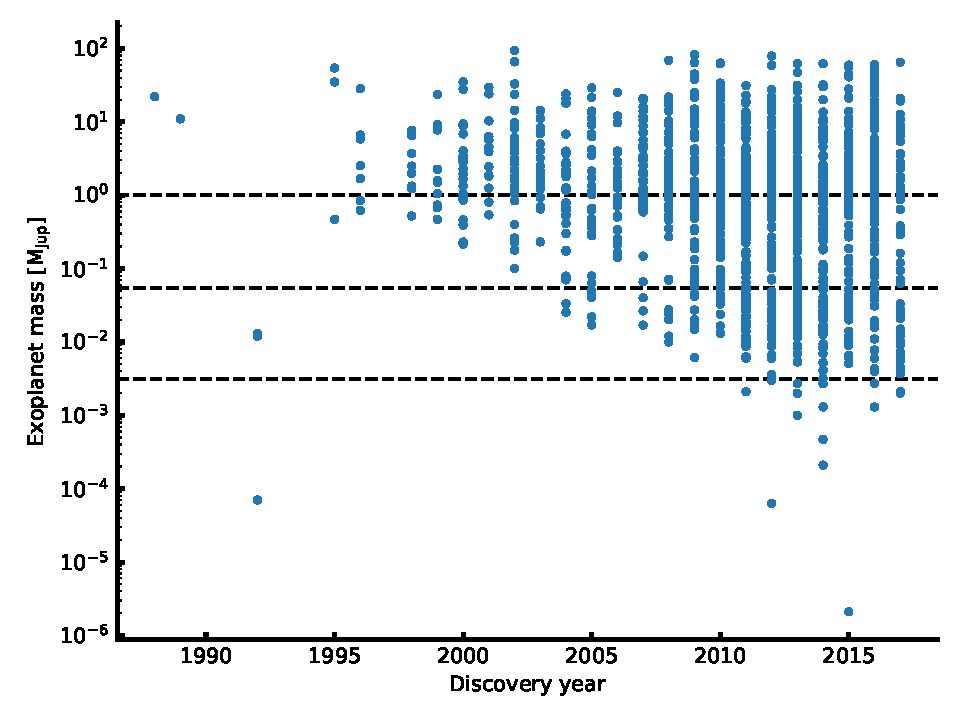
\includegraphics[width=0.8\linewidth]{figures/exoplanetMass.pdf}
    \caption{The mass of exoplanet since the detection of the first exoplanet until now. The
             horizontal lines indicate the mass of Jupiter (upper), Neptune (middle), and Earth
             (lower).}
    \label{fig:exoplanetMass}
\end{figure}

While the first many discoveries of exoplanets were the (at the time) exotic and strange hot
Jupiter-like exoplanets in close orbits, the time have come to detect exoplanets with both lower
mass and wider orbits. It is crucial to have high precision instruments and long surveys to detect
these exoplanets. Missions as \emph{Kepler} and CoRoT have been excellent for this, since they have
focused on few fields of the sky for a long time.

The first place to naively look for Earth's twin would be in a system similar to our own Solar
system. That means around a G dwarf like our own Sun. However, due to the high surface temperature
of these stars\footnote{Very few effort have been made to look for exoplanets around OB stars as
these are both few in numbers and hostile environments for exoplanets.}, the habitable zone will be
far from the host star \citep[see e.g.][]{Kasting1993}. Indeed, to detect a copy of our own
Sun-Earth system we would need to detect the minute signature of an exoplanet in a \SI{1}{year}
orbit around its host star (a solar twin). For the RV method, this minute signature will be
\SI{10}{cm/s}, while the current level of precision is around \SI{1}{m/s}. These signatures can be
measured with the next generation of ultra stable high resolution spectrographs such as ESPRESSO
\citep{ESPRESSO}. If detected with the transit method, more than one transit is needed, hence this
will take at least two years, and probably even longer. Moreover, this is all assuming that the
geometry of the system aligns in such as way that a transit can even be seen from Earth. The
endeavour to get the follow-up RV afterwards will also be extremely challenging with today's
technology, and only the next generation of instruments will be able to detect these signals. In
conclusion, even with perfect instruments, it will take years to detect an Earth twin around a
Sun-twin with the RV and transit methods.

Therefore, it is not a surprise that an effort has been towards detecting Earth-like planets around
the lightest stars. These stars (M stars) are also colder, hence the habitable zone will be closer
to its host compared to the more massive and hotter stars \citep{Kasting1997}, and ultimately the
period for habitable exoplanets will be shorter. The nature has been kind, since it seems that the M
stars are prone to form rocky planets rather than giant gaseous planets
\citep{Bonfils2013,Delfosse2013}. The shorter period means that the surveys can be shorter for these
exoplanets. Moreover, since the host stars are smaller the signal from a transit will be easier to
detect (see \eref{eq:transit}). Similarly will the RV signal be larger for an Earth-like planet in
the habitable zone around an M star compared to a similar exoplanet around a G star. Both due to the
lower period and due to the lower mass of the host star (see \eref{eq:rv}).

While M stars seems to be the place to look for the Earth's twin, there are still some challenges to
tackle. Foremost is the detailed characterisation of the host star, which are particular troublesome
for these stars. This is something that will be focused on in \sref{sec:planet_host_stars}.

\subsubsection{Detecting biosignatures on an exoplanet}

After successfully detecting a rocky exoplanet in the habitable zone the next step is to detect
biosignatures. The best hope is to indirectly detect life by finding biosignatures
\citep{Kasting2002} in the exoplanet's atmosphere. Transmission spectroscopy and lightcurves in
different pass bands are the techniques to study the atmosphere of exoplanets. In this technique a
spectrum of the host star and exoplanet is obtained during transit, which is later subtracted with a
spectrum of the host star during occultation. Hereby it should be possible to obtain a spectrum of
the atmosphere of the exoplanet, which was done by e.g. \citet{Charbonneau2002}.

An interesting test to look for biosignatures from the Earthshine on the Moon was performed by
\citet{Arnold2002} where they clearly see the blue colour of the Earth's atmosphere due to Rayleigh
scattering. They also observed signatures for oxygen, ozone, and water vapours; all important
biosignatures in a planetary atmosphere supporting life.

These signatures, especially oxygen, are from microorganisms through photosynthesis
\citep[see e.g.][]{Kasting2002}. However, there might be conditions outside the habitable zone which
might sustain life. Here on Earth, extremophiles such as the water bears are known to thrive in
extreme places such as boiling water, acid, ice, etc. This might eventually lead to a new window of
opportunity in the search of extraterrestrial life \citep{Cavicchioli2002}.



\section{Planet host stars}
\label{sec:planet_host_stars}

With the present diversity of exoplanets it becomes increasingly important to get an accurate and
precise characterisation of the exoplanets in order to study them in samples and on an individual
level. An accurate and precise characterisation can give us an idea whether the planet is rocky,
composed of water, gaseous, or some other more exotic combination, \hl{by comparing fitting fixed
density profiles (based on different compositions) to the planetary mass and radius}. As mentioned
above, it is crucial to characterise the host stars in order to characterise the exoplanets. The
host stars discovered so far are mainly FGK dwarf stars, although some are more evolved. This can be
seen in \fref{fig:hostDistribution} where the effective temperature of all host stars are shown
against the luminosity. The colour represents the temperature, while the size of the symbols is a
measure of the radius, or with other words, the evolutionary state. The smallest points are the
dwarf stars.

\begin{figure}[htpb!]
    \centering
    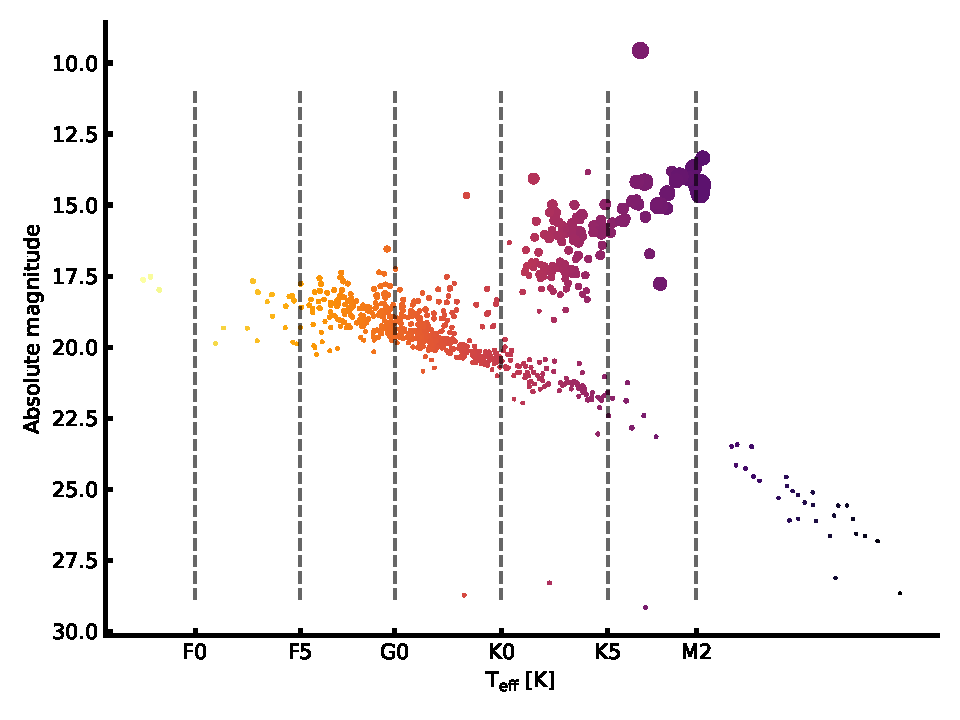
\includegraphics[width=1.0\linewidth]{figures/hostDistribution.pdf}
    \caption{The effective temperature of all host stars are shown against the luminosity. The
             colour represents the temperature, while the size of the symbols is a measure of the
             radius, or with other words, the evolutionary state. The smallest points are the dwarf
             stars. The green star in the plot show the location of the Sun.}
    \label{fig:hostDistribution}
\end{figure}

To make an in-depth characterisation of stars it is common to use several different methods to gain
knowledge about different aspects of a star. If the effective temperature is needed, the reliable
determination comes from the analysis of a high resolution and high signal-to-noise (S/N) spectrum
or the infrared flux method (see \sref{sec:irfm} for more details). Spectroscopy is also used to
identify chemical abundances of the photosphere of the star, while a method like asteroseismology is
used to determine the mass and radius of a star with high precision; two parameters which are
crucial to characterise the orbiting exoplanet.

Some of these methods are described in greater detail in \cref{cha:method}. These methods work best
together. In the example given above, the effective temperature is needed before asteroseismology
can be used to determine the mass and radius. These two methods goes extremely well together as the
most commonly used detection methods (transit and RV) will obtain the data needed. From the transit
method, the obtained lightcurve can be used to detect the transits. If these transits are carefully
removed from the lightcurve, the residual lightcurve might contain stellar oscillations used to
perform an asteroseismic analysis. Likewise will the spectra obtained from the RV method to
detect/confirm an exoplanet be used for the stellar characterising afterwards by combining them,
after shifting to a RV$=\SI{0}{km/s}$, to increase the S/N. This combined high S/N spectrum is ideal
for the spectral analysis of stars.

The synergy between a spectroscopic analysis and asteroseismology have proven very successful
\citep[see e.g.][]{Huber2013} for characterising an exoplanet system (host star and exoplanet).
However, it does have its limitations. It can be difficult to detect solar-like oscillations as the
stars get colder than the Sun. The community has yet to detect any solar-like oscillations in M
dwarf stars \citep{Rodriguez2016,Berdinas2017}. Many of the detected exoplanets are from the
\emph{Kepler} mission, where many of the host stars are very faint. While it is not impossible to
make spectroscopic observations, it is extremely time consuming. Therefore brighter targets are
often prioritised, unless there is an exceptional case.

With the search for the Earth twin around the small cool M dwarf stars, it is important to develop
reliable methods for the analysis of these stars. The tools for detecting the exoplanets are
currently more mature than the host star analysis. However, with the advance of NIR spectrographs
this is slowly changing. It is general believed that a NIR analysis is needed to characterise M
stars. The reason is simple that these stars are so intrinsic faint, that it is important to collect
as much flux as possible. This happens in the NIR. Since M stars are intrinsically faint in the
visible, it is advantageous to use NIR spectrographs where M stars emit most of their light.
Moreover, for spectroscopic studies, the optical spectrum of these stars are severely contaminated
by molecular absorption lines, which depress the continuum. It is crucial to get the continuum
placement correct during spectroscopic studies. In the NIR the continuum depression is less severe,
however still challenging. This can clearly be seen in \fref{fig:opticalVSnir} where the optical and
NIR part of the spectrum for HD 79210, a K7 dwarf star\footnote{Note that there are very little
difference between a K7V and M0V. For the latter case, the situation raised in
\fref{fig:opticalVSnir} will be more clear.}, is plotted. The spectra were obtained by CARMENES
simultaneously and have therefore the same exposure time. During a spectroscopic analysis, which
will be the applied method in this thesis, it is important to observe isolated absorption lines. The
more contaminated and blended a absorption line is, will result in more uncertain results at the end
of the analysis. This will be described in detail in \sref{sec:parameters}. In
\fref{fig:opticalVSnir} it is clear that the NIR spectrum is far less contaminated by absorption
lines.

\begin{figure}[htpb!]
    \centering
    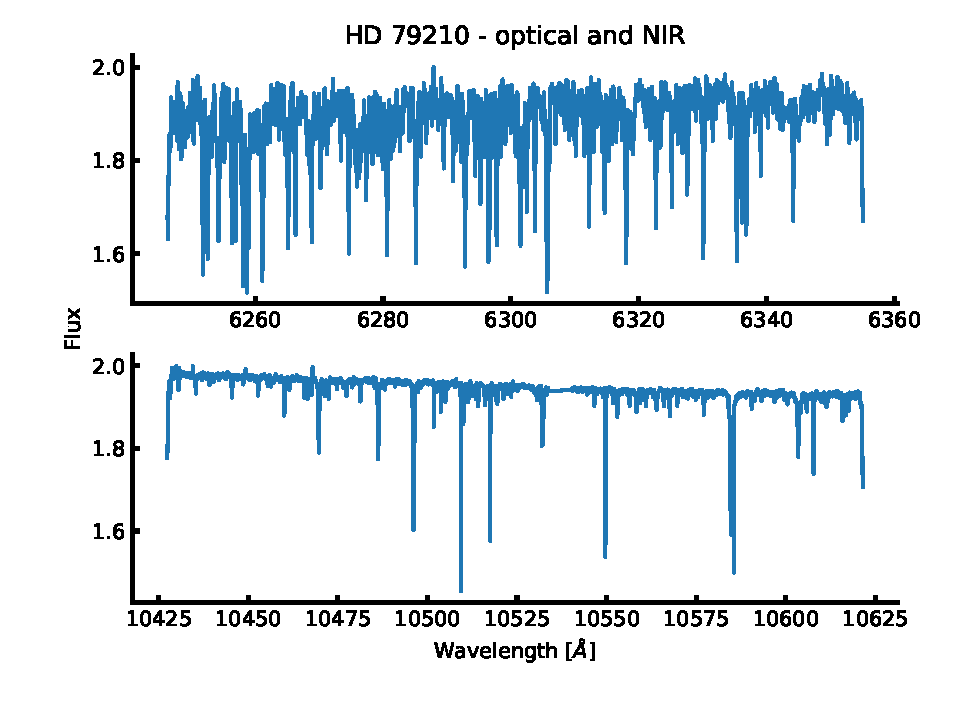
\includegraphics[width=1.0\linewidth]{figures/opticalVSnir.pdf}
    \caption{Comparison between an optical and NIR part of the spectrum of HD 79210 obtained by
             the CARMENES spectrograph. This clearly illustrate why NIR spectra are preferred over
             optical spectra for cool stars, where absorption lines are less blended. HD 79210 is a
             K7 dwarf star.}
    \label{fig:opticalVSnir}
\end{figure}

The main goal of this thesis is to work towards a consistent derivation of stellar atmospheric
parameters for M stars. Before tackling the M stars, it is important to have a method that work well
for solar-like stars (FGK), which are better known during countless studies.

\subsection{Star-planet correlations}

While the stellar parameters are used to determine the planetary parameters, they can also be sued
to reveal correlations between planets and their host stars. This might give insight in the
formation and evolution of the planets. Indeed, several important correlations have been found
already.

\paragraph{Giant planet and metallicity correlation}

Since the first discoveries of exoplanets, it became evident that giant planets were systematically
orbiting more metal-rich stars compared to stars with no planets. This correlation have been
confirmed by several studies \citep{Gonzalez1997,Santos2004,Fischer2005,Sousa2008a,Mortier2013b}
\hl{ and can be seen in} \fref{fig:fehCorrelation} \hl{using the data from} \citet{Sousa2008a}. This
correlation in turn establish that core accretion is the main formation mechanism among giant
exoplanets \citep{Pollack1996,Ida2004,Mordasini2012} and not disc instability \citep{Boss2002}.

\begin{figure}[htpb!]
    \centering
    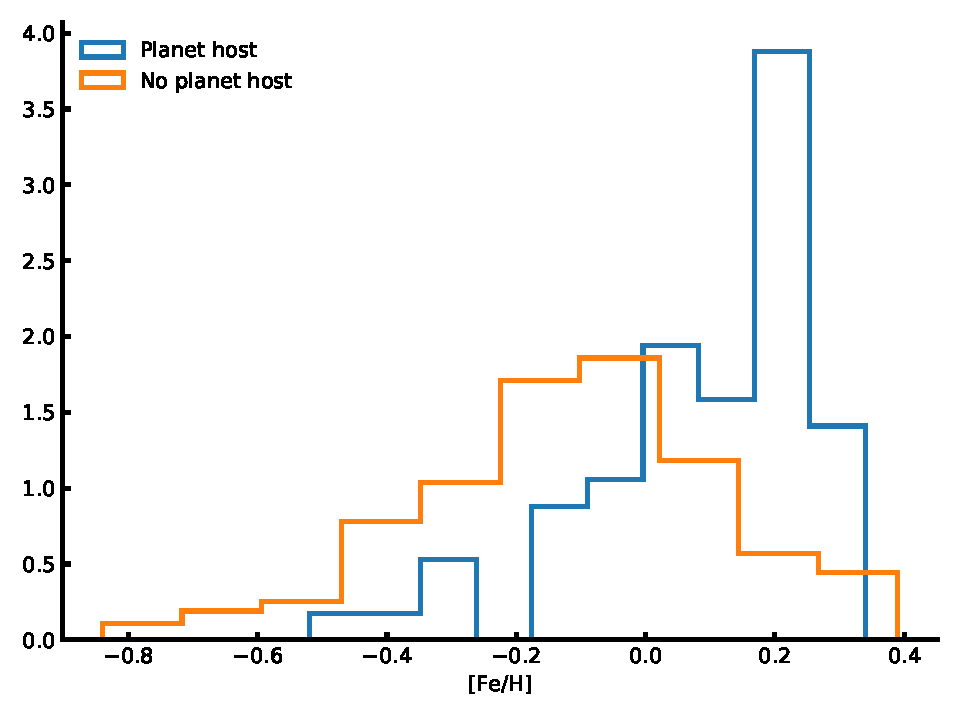
\includegraphics[width=1.0\linewidth]{figures/fehCorrelation.pdf}
    \caption{Metallicity correlation for giant planets, comparing planet hosts and non host stars
             from the sample of \citet{Sousa2008a}. It is clear that planet host stars have higher
             metallicities than non hosting stars. The histograms are normalized.}
    \label{fig:fehCorrelation}
\end{figure}

It is important to note that recent studies find this correlation for Neptune-like and
super-Earth planets as well \citep{Wang2015,Zhu2016}.

However, some new observational evidence \hl{show two giant exoplanet populations}
\citep{Santos2017}, \hl{one which} \st{may} favour disc instability \citep[see e.g.][]{Nayakshin2017}.

\paragraph{Abundances of heavy elements}

It has been shown that metal-poor stars harbouring gas planets are enhanced in alpha
elements\footnote{These are elements formed by fusion of a helium core; C, N, O, Ne, Mg, Si, S, Ar,
Ca, and Ti.} \citep[see e.g.][]{Adibekyan2012a}. This means that other elements than iron also have
a role to play in planet formation in iron-poor environments.


\paragraph{Lithium and the presence of planets}

It has been shown by \citet{Israelian2004,Delgado2014,Gonzalez2015,Takeda2005} that stars hosting
planets are significantly more \ion{Li}{} depleted compared to stars without planets. This
correlation seems to be physically related with the occurrence of planets and not e.g. age, mass, or
metallicity of the stars \citep{Sousa2010}. Other studies does not find any correlation between
\ion{Li}{} depletion and stars with planets \citep{Baumann2010,Ramirez2012}.



\section{Applications from knowing the stars}
\label{sec:stars_application}

While ``know the star, to know the exoplanet'' is the main motivation behind this thesis, it is
obviously not the only application behind detailed stellar characterisation. Working towards a
better understanding of especially M stars, which consist of to 70\% of all the stars in the Milky
Way \citep{Bochanski2010}, will also open a new window into the study of different galactic
components and galactic chemical evolution. Such a study was done by e.g.
\citet{Adibekyan2012,Delgado2017} where spectra of 1111 FGK dwarf stars from the HARPS GTO sample
was used to derive chemical abundances of 12 refractory elements. It is possible to separate
different galactic populations (thin disk, thick disk, and the halo) by studying the chemical
abundances of stars as was shown in \citet{Adibekyan2012}.

In order to do a detailed chemical analysis\footnote{See also references within
\citet{Adibekyan2012} for other similar studies.}, it is crucial to have reliable and homogeneously
derived stellar atmospheric parameters. If the parameters are homogeneously derived, i.e. with the
same method, one does not need to worry about removing possible offsets when joining results from
different methods, and in case of known offsets it is easy to correct for them (this is the case for
the method used throughout this thesis, where the surface gravity will be corrected based on another
method).


\section{This thesis}
\label{sec:this_thesis}

This thesis will be focused on deriving stellar atmospheric parameters for FGK stars, making the
bridge towards M stars. This task will be accomplished utilising high resolution and high S/N NIR
spectra. The theory of stellar atmospheres in a nutshell is described in \cref{cha:theory}, setting
up all the tools to derived them as described in \cref{cha:method}. In \cref{cha:method} the
description of other useful and commonly used methods for deriving parameters are also presented.
Thereafter the knowledge will all be used in \cref{cha:results}. First by obtaining a NIR line list
containing \ion{Fe}{I} and \ion{Fe}{II} lines, then by the derivation of parameters for HD 20010 (F
sub-giant). Before deriving parameters for two K giants, the NIR line list will be revisited.

After focusing on the NIR spectra, the optical counterpart of the method described below will be
used to derive parameters for 50 planet-host stars for an online catalogue of homogeneously derived
parameters (SWEET-Cat) in \cref{cha:SWEET-Cat}.

Last in \cref{cha:future} the future of the work established here will be discussed along with the
results already obtained. This will round of the thesis.

After the last chapter there will be a few appendices with large tables that would otherwise
distract the reader from the main points. One appendix, \cref{cha:fasmaML}, will be on derivation of
stellar atmospheric parameters using machine learning, which was a side project during the thesis.
This appendices are followed by the bibliography for this thesis.
